\documentclass[border=4pt]{standalone}
\usepackage{amsmath,amssymb,tikz}
\usetikzlibrary{arrows.meta,calc,decorations.markings}
\begin{document}
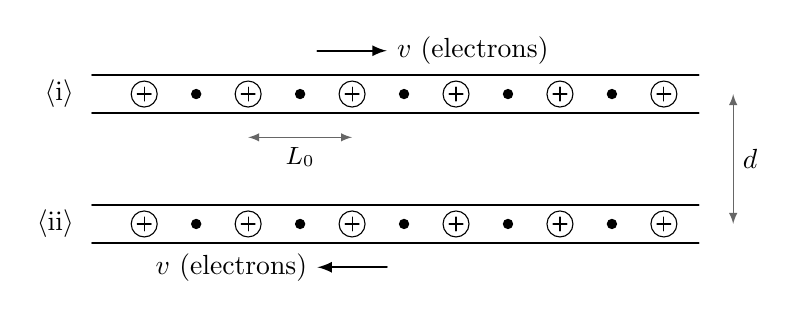
\begin{tikzpicture}[scale=1.1,>=latex,line cap=round]
  \foreach \y/\lab/\dir in {1.5/i/1,0/ii/-1}{
    \draw[thick] (0,\y+0.22) -- (7,\y+0.22); \draw[thick] (0,\y-0.22) -- (7,\y-0.22);
    \foreach \x in {0.6,1.8,3.0,4.2,5.4,6.6}{\draw (\x,\y) circle (0.15); \draw (\x-0.08,\y)--(\x+0.08,\y); \draw (\x,\y-0.08)--(\x,\y+0.08);}
    \foreach \x in {1.2,2.4,3.6,4.8,6.0}{\fill (\x,\y) circle (0.06);}
    \node[left] at (-0.1,\y) {$\langle\text{\lab}\rangle$};
  }
  \draw[->,thick] (2.6,2.0) -- (3.4,2.0) node[right]{$v$ (electrons)};
  \draw[->,thick] (3.4,-0.5) -- (2.6,-0.5) node[left]{$v$ (electrons)};
  \draw[<->,black!60] (7.4,1.5) -- (7.4,0) node[pos=0.5,right,black]{$d$};
  \draw[<->,black!60] (1.8,1.0) -- (3.0,1.0) node[pos=0.5,below,black,font=\small]{$L_0$};
\end{tikzpicture}
\end{document}
